\chapter{Concept - Representing Information with Symbols}
\label{chapter:representingInformationWithWymbols}

\section{Similar Words}
\label{section:similarWords}

Representing information with symbols is a fundamental concept of Computer Science as information should be displayed clearly and concisely. Words can be seen as a sequence of symbols, namely a sequence of letters. The examples given in this section are in German, since the final application is in German as well.

In order to transmit information, it needs to be encoded in a word and sent to the destination.  The receiver needs to be able to decode and make sense of the transmitted information, even tough the word might contain errors such as spelling mistakes. To achieve this, sender and receiver agree on a list of used words. Each pair of words from this list has a minimal editing distance. 

The editing distance is the amount of operations that need to be done to transform a word in another by applying a sequence of operations. The operations are deleting, inserting and changing a letter \cite{AnD}.

\begin{example}
    The editing distance between \code{BACH} and \code{FACH} is 1, since changing the first letter from \code{B} to \code{F} transforms the first word into the second.
\end{example}

If sender and receiver agree on a list of words with a minimal pairwise editing distance and to only transmit words from this list, then the receiver can still uniquely determine what word the sender has sent, even when an error has been made. The receiver calculates the minimal editing distance between the received word and each word of the list and chooses the word with the smallest editing distance. The receiver assumes that this was the word the sender originally sent.

\subsection{Exercises}

The purpose of the \nameref{section:similarWords} exercises is to learn particular operations. An exercise is dedicated to one of the following operations: adding, changing and removing a letter from a word. Additionally, an exercise about swapping adjacent letters in a word is included.

\subsection*{Adding a letter}
\label{subsection:addingLetter}

In the \nameref{subsection:addingLetter} exercise, pupils are presented a word and the alphabet from A to Z. Pupils are supposed to choose a letter from the alphabet and add it to the word to form a new valid word.

\begin{example}
    The word \code{ARM} is given. By adding the letter \code{D} before the first letter, the valid word \code{DARM} is formed.
\end{example}

\subsection*{Changing a letter}
\label{subsection:changingLetter}

In this exercise, pupils are again shown a word and the alphabet from A to Z. The pupils should select a letter from the alphabet, but this time, instead of adding it, the selected letter should replace a letter from the word itself to create a new valid word.

\begin{example}
    The word \code{BUCH} is given. By changing the first letter from \code{B} to \code{T} the new valid word \code{TUCH} is formed.
\end{example}

\subsection*{Removing a letter}
\label{subsection:removingLetters}

In the \nameref{subsection:removingLetters} exercise, pupils receive a word, from which they should remove a letter to form a new valid word.

\begin{example}
    The word \code{BAUCH} is given. By removing the third letter the new valid word \code{BACH} is formed.
\end{example}

\subsection*{Swapping adjacent letters}
\label{subsection:swappingLetters}

When typing on a keyboard, typing mistakes happen. This exercise is supposed to train the ability to spot a common mistake, where only two adjacent letters are swapped \cite{EinfachInformatik}.

The pupils are presented a word with swapped adjacent letters, which they need to identify and swap back to restore the original word. This exercise has two difficulty levels. On the easy level only one pair of adjacent letters is swapped and on the medium level two pairs of adjacent letters are swapped.

\begin{example}
    The word \code{BCAH} is given (easy level). By swapping the second and third letter the original word \code{BACK} is restored.
\end{example}

\subsection{Implementation}

\subsection*{Word List Generation}

The foundation of these exercises is to have a list of words and for each word a list of similar words. A similar word is a word into which the original word can be transformed by either adding, changing or removing letters within a given number of operations, i.e. editing distance. In this implementation the editing distance used is one. This means only one operation can be applied, either adding, changing or removing a letter. This makes generating a list of words the easy part. Basically any list of words will do the job, but they should be understandable for children. So the first step is to collect a list of child-friendly nouns. 

Not much more difficult, but much more expensive, is the computation of similar words. Given the list of child-friendly nouns and the list of allowed words, one can brute force a list of similar words by applying each transformation to every noun and checking whether the transformed word exists in the allowed word lists. The script to generate a list of similar words for each word and each operation is given in listing \ref{lst:similarWords}.

%TC:ignore
\begin{lstlisting}[language=Python,caption={Algorithm to generate a list of similar words in Python},label={lst:similarWords}]
for word in children_words:
  add = list()
  for pos in range(len(word) + 1):
    for letter in ALPHABET:
      w = word[:pos] + letter + word[pos:]
      if contains(allowed_words, w) and not w in add:
        add.append(w.upper())
  similar_words["add"][1][word.upper()] = add

  remove = list()
  for pos in range(len(word)):
      w = word[:pos] + word[pos + 1 :]
      if contains(allowed_words, w) and not w in remove:
          remove.append(w.upper())
  similar_words["remove"][1][word.upper()] = remove

  change = list()
  for pos in range(len(word)):
    for letter in ALPHABET:
      w = word[:pos] + letter + word[pos + 1 :]
      if w != word and contains(allowed_words, w) and not w in change:
        change.append(w.upper())
  similar_words["change"][1][word.upper()] = change

  change = list()
  for left_pos in range(len(word)):
    for right_pos in range(left_pos + 1, len(word)):
      for left_letter in ALPHABET:
        for right_letter in ALPHABET:
          if word[left_pos] == left_letter or word[right_pos] == right_letter:
            continue
          w = (
            word[:left_pos]
            + left_letter
            + word[left_pos + 1 : right_pos]
            + right_letter
            + word[right_pos + 1 :]
          )
          if w != word and contains(allowed_words, w) and not w in change:
            change.append(w.upper())
  if len(change) >= MIN_SIMILAR_WORDS:
    change.sort()
    similar_words["change"][2][word.upper()] = change
\end{lstlisting}
%TC:endignore

\begin{example}
  Examples of similar words for adding, changing and removing a letter from a word
  \begin{itemize}
    \item \nameref{subsection:addingLetter} - \code{ARM}: \code{ARME}, \code{ARMS}, \code{DARM}, \code{FARM}, \code{WARM}
    \item \nameref{subsection:changingLetter} - \code{BUCH}: \code{AUCH}, \code{BACH}, \code{BUSH}, \code{EUCH}, \code{HUCH}, \code{SUCH}, \code{TUCH}
    \item \nameref{subsection:removingLetters} - \code{BAUCH}: \code{AUCH}, \code{BACH}, \code{BUCH}
  \end{itemize}
\end{example}

Significantly more difficult is to generate a list of allowed words. Three different approaches were taken:

\begin{itemize}
  \item Using a list of approximately ten thousand nouns
  \item Collecting a list from online dictionary of allowed words of the well known word game Scrabble \cite{Scrabble}
  \item Generating a list from a spell checker
\end{itemize}

The first approach resulted in a word list with which exercises could be generated. However, the word list obviously didn't cover all possible words pupils could know. Therefore, the word list needed to be extended.

Hence the idea to create a list of words that are allowed in Scrabble came up. This seemed like a good idea until it showed that the online Scrabble dictionary does not include all valid words.
Collecting words from the Scrabble dictionary resulted in approximately thirty thousand words, each between two and 8 letters long.

Finally, the last approach was taken by generating a list of allowed words from a spell checker. A well-known and open-source spell checker is Hunspell. However, Hunspell doesn't have a list of all allowed words, but rather generates them from two files: the dictionary file and the affix file. The dictionary file contains a list of root words and applicable rules for each root word. The affix file stores a list explaining these rules. Each rule defines an operation that can be applied to a root word. The spell checker evaluates a word as correct if it can construct the word by applying rules to a root word \cite{Hunspell}.

Luckily, there exists a tool called \code{unmunch} in the Hunspell ecosystem that generates a list of words from the dictionary file and the affix file as easy as shown in listing \ref{lst:unmunch} \cite{HunspellGithub}.
In the end, a list of about one million allowed words was generated (without any word length limits). However, a drawback is that the word list does not contain any names from people, cities or any other instances. 

%TC:ignore
\begin{lstlisting}[language=Bash,caption={Bash command to unmunch a dictionary file and a affix file to a list of words},label={lst:unmunch}]
$ unmunch German_de_CH.dic German_de_CH.aff > wordlist.txt
\end{lstlisting}
%TC:endignore

The actual implementation of these exercise types is straight forward. Each exercise type displays a random word from the word list and each letter of the word is on a card to allow easy user interaction. Two exercise types, namely adding and changing a letter, need an alphabet. The \nameref{subsection:addingLetter} exercise is implemented in the \code{Add.vue} component (figure \ref{fig:addingLetter}) and shows arrows between each letter and at the beginning and end of the word, where pupils can add a new letter selected from the alphabet. The \nameref{subsection:changingLetter} exercise works similarly, but instead of having arrows, pupils can replace each letter themselves with a new letter selected from the alphabet (figure \ref{fig:changingLetter}). In the \nameref{subsection:removingLetters} exercise, pupils can move a letter to the trashcan to remove it (figure \ref{fig:removingLetter}). In the \nameref{subsection:swappingLetters} exercise, they can click on the arrows to change the order of the letters (figure \ref{fig:swappingLetters}).

\begin{figure} 
  \centering
  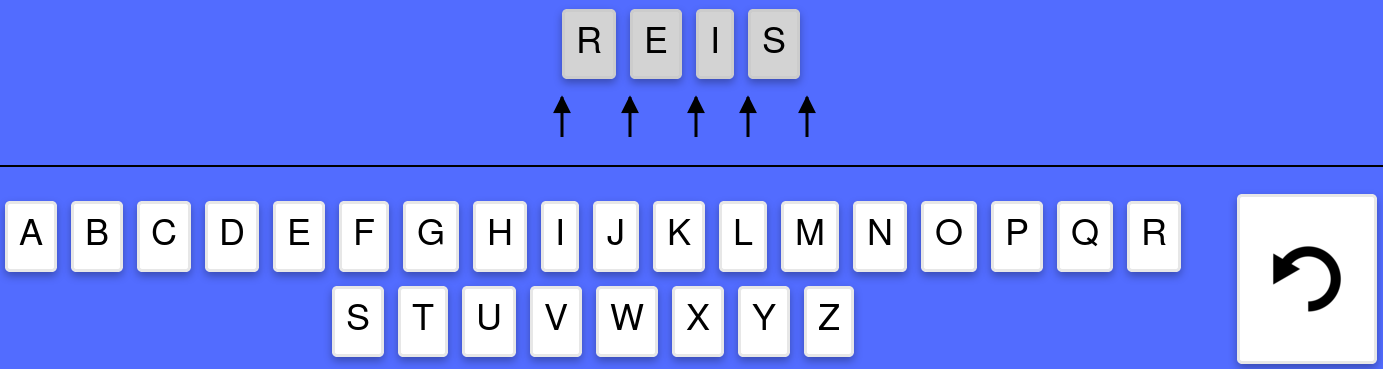
\includegraphics[width=1.0 \columnwidth]{figures/words_add.png}
  \caption{Adding a letter exercise} 
  \label{fig:addingLetter} 
\end{figure}

\begin{figure} 
  \centering
  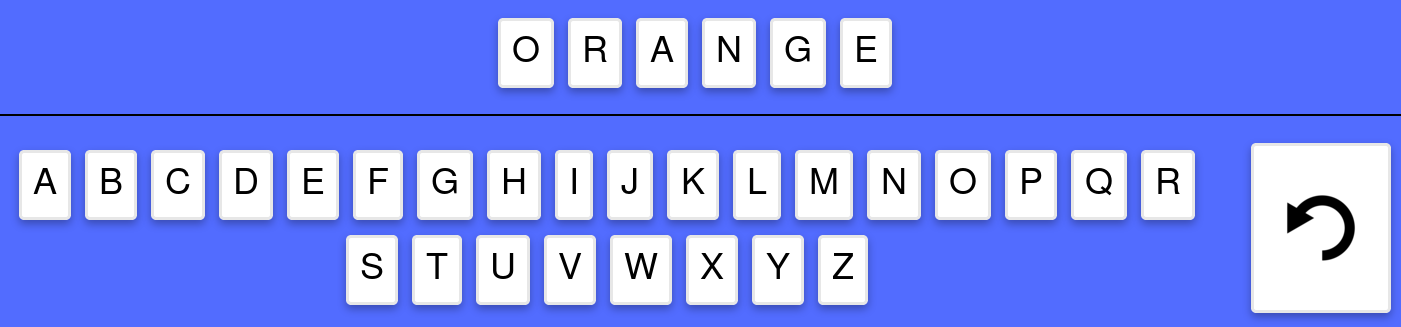
\includegraphics[width=1.0 \columnwidth]{figures/words_change.png}
  \caption{Changing a letter exercise} 
  \label{fig:changingLetter} 
\end{figure}

\begin{figure} 
  \centering
  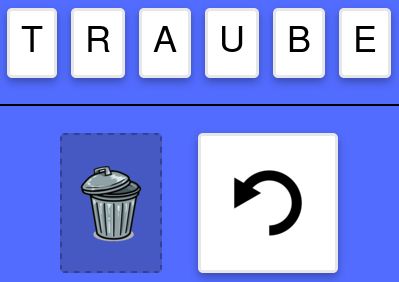
\includegraphics[width=0.3 \columnwidth]{figures/words_remove.png}
  \caption{Removing a letter exercise} 
  \label{fig:removingLetter} 
\end{figure}

\begin{figure} 
  \centering
  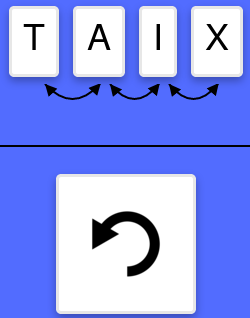
\includegraphics[width=0.2 \columnwidth]{figures/words_swap.png}
  \caption{Swapping letters exercise} 
  \label{fig:swappingLetters} 
\end{figure}

\section{Number Systems}
\label{section:numberSystems}

\subsection{Exercises}
\subsection*{Representing Numbers like the Maya}

Today, people are used to the decimal number system (base number 10), with 10 symbols. The Maya used a different number system with a base number of 20 i.e the vigesimal number system. It is believed that the Maya used their ten fingers and ten toes to count adding up to twenty. But instead of having a symbol for each number as in the decimal system, the Maya used three different symbols: zero (a turtle shell, belly side up), one (a dot) and five (a bar) \cite{Maya}. The Mayan representation of the decimal numbers from 0 to 19 can be found in figure \ref{fig:maya_numerals}.

\begin{figure} 
    \centering
    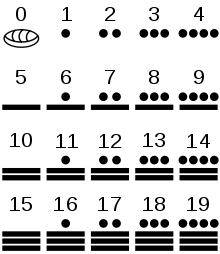
\includegraphics[width=0.3 \columnwidth]{figures/maya_number_system.png}
    \caption{Representation of the Maya numbers from 0 to 19} 
    \label{fig:maya_numerals} 
\end{figure}

The following exercises are supposed to familiarize pupils with a new number system, the Mayan number system. First, converting numbers between the decimal number system and the Mayan numbers is trained and then topped off with an exercise about adding two Mayan numbers.

\subsubsection*{Representing Mayan numbers}

A decimal number is presented to the pupils. They need to choose the correct amount of dots and bars representing the decimal number as shown in figure \ref{fig:maya_numerals}. For the purpose of simplicity, only decimal numbers between 1 and 19 are chosen.

\subsubsection*{Understanding Mayan numbers}

In this exercise the pupils learn to understand Mayan numbers. Again only decimal numbers between 1 and 19 are used. The pupils need to understand what Mayan number is shown and write down the decimal equivalent.

\subsubsection*{Adding Mayan numbers}

This exercise combines the previous two. The pupils need to understand the summands given in the Mayan number system, add them together and write down the sum in either the decimal number system or the Mayan number system. This exercise has two difficulty levels:

\begin{itemize}
  \item \textbf{easy} - the pupils have to calculate the sum as a number 
  \item \textbf{medium} - the pupils have to calculate the sum as a representation of numbers from the Mayan number system
\end{itemize}

\subsection*{Representing Numbers with Coins}

The following exercises introduce a new number system and train an already learned one: the binary number system and the decimal number system. Both number systems are practiced with coins and with numbers. The binary coins include the following numbers: 1, 2, 4, 8, 16, 32 and 64 (figure \ref{fig:binary_coins}). The decimal coins include 1, 2, 5, 10, 20 and 50 (figure \ref{fig:decimal_coins}). 
Overall, the same concepts are practiced for both number systems with the limitation that every binary coin can at most be used once.

\begin{figure} 
    \centering
    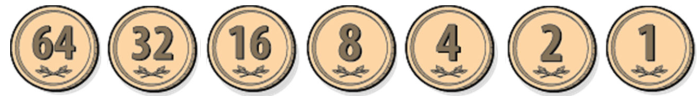
\includegraphics[width=0.5 \columnwidth]{figures/decimal_coins.png}
    \caption{Representation of the decimal coins} 
    \label{fig:decimal_coins} 
\end{figure}

\begin{figure} 
    \centering
    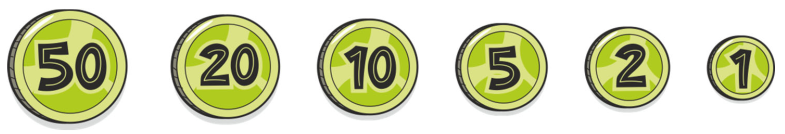
\includegraphics[width=0.5 \columnwidth]{figures/binary_coins.png}
    \caption{Representation of the binary coins} 
    \label{fig:binary_coins} 
\end{figure}

\subsubsection*{Conversion of a decimal number to its coin representation}

This exercise includes two difficulty levels:

\begin{itemize}
    \item Converting a decimal number to a coin representation, where the sum of all coins are equal to the decimal number
    \item Converting a decimal number to a coin representation, where the sum of all coins are equal to the decimal number \textbf{and} the amount of used coins is minimal.
\end{itemize}

\subsubsection*{Conversion of a number given in its coin representation to a decimal number}

A number given in its coin representation, either binary or decimal coins, has to be converted to a decimal number. 

\subsubsection*{Reducing the amount of used decimal coins while keeping the same sum}

Similar to the previous exercise, a sum in its coin representation is given and pupils have to display the same sum but with fewer coins. This exercise only makes sense for decimal coins since binary coins are always minimal.

\subsection{Implementation}

The conversion exercises from the decimal number system to either the Mayan, decimal coins or binary coins all share the same logic implemented in the \code{To.vue} component (figure \ref{fig:coinsTo}).
The same goes for the inverse direction (\code{From.vue} component, figure \ref{fig:coinsFrom}).
However, adding Maya numbers (\code{Addition.vue}, figure \ref{fig:mayanAddition}) and reducing the amount of used coins (\code{Swap.vue}, figure \ref{fig:coinsSwap}) require their own logic and are therefore implemented in their own components.

\begin{figure} 
  \centering
  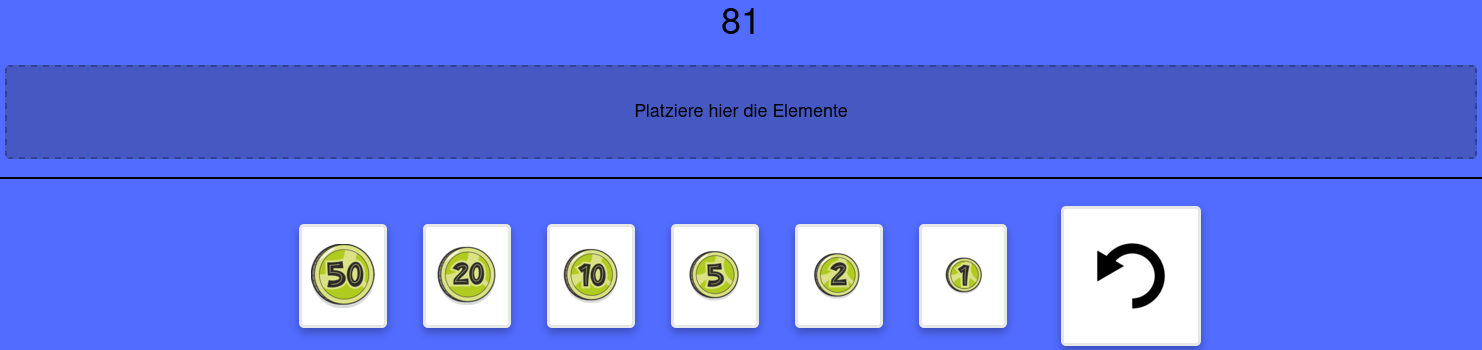
\includegraphics[width=1.0 \columnwidth]{figures/coins_to.png}
  \caption{Conversion of a decimal number to its coin representation exercise} 
  \label{fig:coinsTo} 
\end{figure}

\begin{figure} 
  \centering
  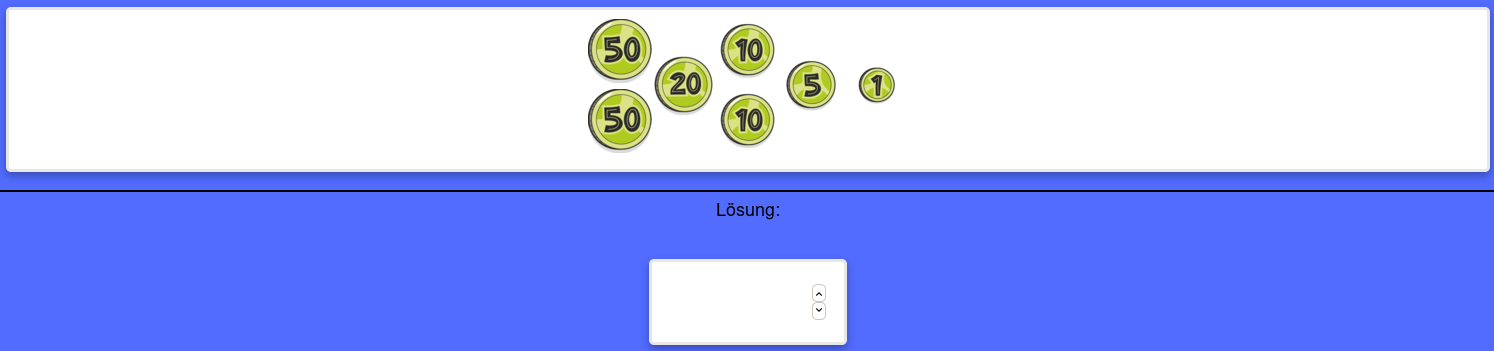
\includegraphics[width=1.0 \columnwidth]{figures/coins_from.png}
  \caption{Conversion of a decimal number from its coin representation exercise} 
  \label{fig:coinsFrom} 
\end{figure}

\begin{figure} 
  \centering
  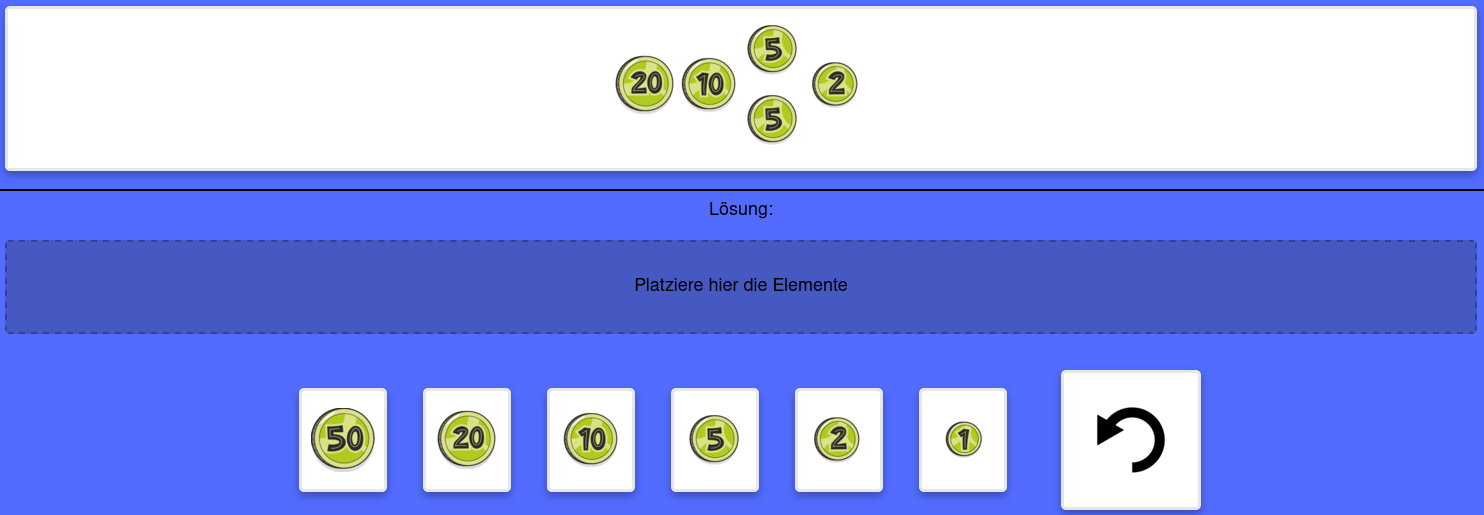
\includegraphics[width=1.0 \columnwidth]{figures/coins_swap.png}
  \caption{Reducing the amount of decimal coins in a given set of decimal coins exercise} 
  \label{fig:coinsSwap} 
\end{figure}

\begin{figure} 
  \centering
  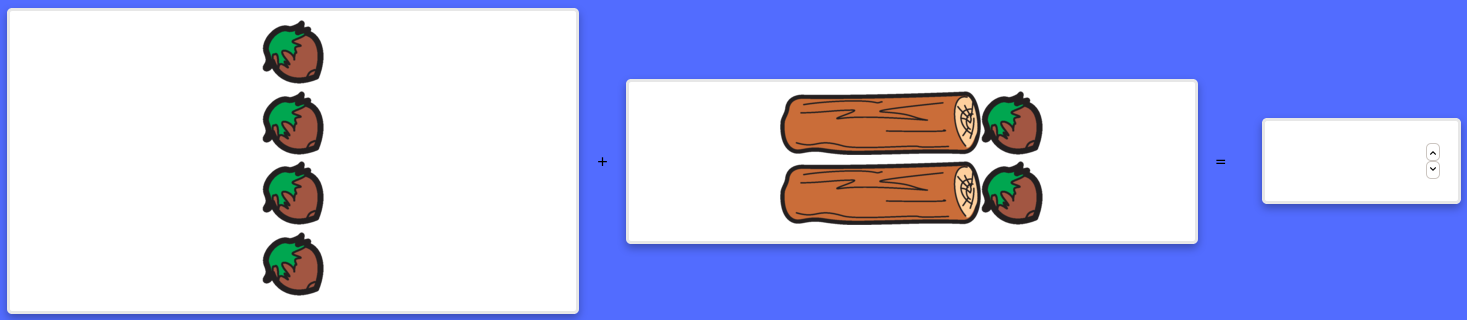
\includegraphics[width=1.0 \columnwidth]{figures/mayas_addition.png}
  \caption{Adding Mayan numbers exercise (easy)} 
  \label{fig:mayanAddition} 
\end{figure}

The \code{To.vue} component is simple. It shows a a random number between one and a number system specific limit:

\begin{itemize}
  \item \textbf{Mayan number system} - limit: 19
  \item \textbf{Decimal coins} - limit: 100
  \item \textbf{Binary coins} - limit: 100
\end{itemize}

The pupils need to select items (either nuts, sticks or coins) with the correct value and place them such that they sum up to the shown random number.
In addition, there is another difficulty level for the conversion to decimal coins, where the aim is to represent the displayed random number with as few decimal coins as possible. The algorithm to calculate the minimal amount of items necessary for a certain sum is given in listing \ref{lst:calcMinimalAmount} 


%TC:ignore
\begin{lstlisting}[language=TypeScript,caption={Calculate minimal amount of items needed to reach a certain number},label={lst:calcMinimalAmount}]
calcMinimalAmount(type: numbersystemType, number: number): number[] {
  const items = this.items(type);
  let i = 0;
  const minimalAmount = new Array<number>(items.length).fill(0);
  while (number > 0 && i < items.length) {
    const value = items[i].value;
    if (number >= value) {
      minimalAmount[i]++;
      number -= value;
    } else {
      i++;
    }
  }
  return minimalAmount;
}
\end{lstlisting}
%TC:endignore

The implementation for the \code{From.vue} component works in a similar fashion. This time a random number of items is generated. The pupils need to add up these items' values.

Both of these components at some point need to sum the items' values. It would be convenient to have a map where each item type maps to the amount of selected or shown items and a map where each item type maps to its value. However, due to Vue.js constraints, this is not possible, as the Map datatype is not reactive.

The Array datatype on the other hand is reactive. Therefore an array is used, where the first element represents the highest item value, and the last element represents the item with the lowest value. This introduces some tight coupling between the array storing the amount of items and the array storing the value of each item. The implementation to sum items is shown in listing \ref{lst:sumItems}.

%TC:ignore
\begin{lstlisting}[language=TypeScript,caption={Sum up items},label={lst:sumItems}]
sumItems(type: numbersystemType, items: number[]): number {
  if (items.length !== this.items(type).length) {
    throw Error(`array lengths do not match:  ${items} ${this.items(type)}`);
  }
  let sum = 0;
  for (let i = 0; i < this.items(type).length; i++) {
    sum += items[i] * this.items(type)[i].value;
  }
  return sum;
}
\end{lstlisting}
%TC:endignore

The \code{Swap.vue} component reuses some parts of the just mentioned components. It also generates a random amount of each item. The total amount of items is guaranteed to be reducible and pupils are asked to represent the same sum over all items but with fewer items. How such a configuration is achieved, is shown in listing \ref{lst:reducableItems}.

%TC:ignore
\begin{lstlisting}[language=TypeScript,caption={Generate a reducible item configuration},label={lst:reducableItems}]
do {
  this.generatedItems = this.generateItems(this.type);
} while (
  this.sumItems(this.type, this.generatedItems) >= this.limit(this.type) ||
  this.countItems(this.generatedItems) ===
    this.countItems(
      this.calcMinimalAmount(
        this.type,
        this.sumItems(this.type, this.generatedItems)
      )
    )
);
\end{lstlisting}
%TC:endignore

In the \code{Addition.vue} component all previously seen concepts come together. Two summands are generated, each with a random amount of items. The sum is guaranteed to not overshoot the limit of this number system. 